%\documentclass[dvipdfmx]{beamer}
\documentclass{beamer}                   % lualatex の場合
\usepackage{mySld}

\begin{document}
\title[二次記憶装置]
      {オペレーティングシステム\\第14章 二次記憶装置}
\date{}
\begin{frame}
  \titlepage
  \centerline{\url{https://github.com/tctsigemura/OSTextBook}}
\end{frame}

%\section{}
%=========================================================================
%\begin{frame}
%  \frametitle{}
%\end{frame}

\section{二次記憶装置}
%=========================================================================
\begin{frame}
  \frametitle{記憶装置の階層(1)}
  \fig{scale=1.3}{memoryHierarchy.pdf}
  \begin{itemize}
  \item \emph{レジスタ}はCPUレジスタのこと.\\
    容量は数十バイト程度,高速アクセスが可能,揮発性
  \item \emph{主記憶(メモリ)} \\
    アクセス時間は数ナノ秒〜十数ナノ秒程度\\
    容量は数Giバイト〜数十Giバイト程度,揮発性
  \item \emph{二次記憶装置} \\
    ハードディスクやSSD(Solid State Drive)のこと.\\
    アクセス時間は数ミリ秒〜数十ミリ秒(ハードディスク),不揮発性
\end{itemize}
\end{frame}

%=========================================================================
\begin{frame}
  \frametitle{記憶装置の階層(2)}
  夫々の特性に合った使い方をする.\\
  \emph{二次記憶装置の特性}は次の通り.
  \begin{itemize}
  \item 大容量(ビット単価が安い)\\
    オペレーティングシステム,アプリケーション,データなどの\\
    全てを格納できる.
  \item 不揮発性(電源を切っても消えない) \\
    プログラムやデータの永続的な置き場所として適している.
  \end{itemize}
  \vfill
\end{frame}

%=========================================================================
\begin{frame}
  \frametitle{二次記憶装置の種類(1)}
  \fig{scale=0.4}{hardBlock-crop.pdf}
  \emph{接続方式}
  \begin{itemize}
  \item CPUからはホストコントローラを介してアクセスする.
  \item 二次記憶装置はSATAやUSBバスの先に接続される.
  \item USBメモリスティックやポータブルハードディスクは取り外し可能.
  \item 取り外し可能 => データ交換,バックアップ用途にも適する.
  \end{itemize}
\end{frame}

%=========================================================================
\begin{frame}
  \frametitle{二次記憶装置の種類(2)}
  \fig{scale=0.2}{magneticTape.jpg}
  \emph{テープ型装置}
  \begin{itemize}
  \item データのバックアップや輸送用(ビット単価が安い)
  \item \emph{シーケンシャルアクセス}専用
  \item 読み出し位置まで進むために数分!!
  \end{itemize}
\end{frame}

%=========================================================================
\begin{frame}
  \frametitle{二次記憶装置の種類(3)}
  \fig{scale=0.2}{hardDisk.jpg}
  \emph{ディスク型装置}
  \begin{itemize}
  \item \emph{ランダムアクセス}が可能
  \item ハードディスクのこと(CD-ROMなどの光ディスクも仲間)
  \item SSD,USBメモリ,その他メモリカードも仲間
  \end{itemize}
\end{frame}

%=========================================================================
\begin{frame}
  \frametitle{ハードディスク(1)}
  \fig{scale=0.2}{hardDisk.jpg}
  \begin{itemize}
  \item システムの起動ドライブ(OS,アプリ,データ全てが置かれる)
  \item 仮想記憶のバックストレージとしても使用される.
  \item ハードディスク管理が,OSの性能や使い勝手を左右する.
  \item ファイル管理機構はハードディスクを前提にしていることが多い
  \end{itemize}
\end{frame}

%=========================================================================
\begin{frame}
  \frametitle{ハードディスク(2)}
  \fig{scale=0.2}{hardDisk.jpg}
  \emph{セクタ・トラック・シリンダ}
  \begin{itemize}
  \item 同心円の\emph{トラック(Track)}
  \item トラックを区切った\emph{セクタ(Sector)}
  \item トラックをまとめた\emph{シリンダ(Cylinder)}
  \end{itemize}
\end{frame}

%=========================================================================
\begin{frame}
  \frametitle{ハードディスク(3)}
  \emph{セクタのアドレッシング}\\
  512バイト(4KiB)のセクタのアドレス付け方法
  \begin{itemize}
  \item \emph{CHS(Clinder Head Secor)}方式
    \begin{itemize}
    \item Clinder Head Secor の三次元アドレス.
    \item Head は Track と同じ意味.
    \item CHSはPCの世界で使用されてきた用語.
    \item ハードディスクの物理的な構造通りのアドレッシング.
    \item 過去,長く使われてきた方式.
  \end{itemize}
  \item \emph{LBA(Logical Block Addressing)}
    \begin{itemize}
    \item セクタの通し番号(一次元)を用いる.
    \item ハードディスクブラックボックス化(物理構造通が不明)
    \item CHSは煩雑なだけでメリットがなくなった.
    \end{itemize}
  \end{itemize}
\end{frame}

%=========================================================================
\begin{frame}
  \frametitle{フォーマッティング(1)}
  \emph{ハードディスクの初期化の例}
  \begin{itemize}
    \item[1.] 低レベル(物理)フォーマット \\
      ディスクの表面に磁気的にトラックを書き込む.
    \item[2.] \emph{パーティション}(区画)に分割 \\
      \begin{itemize}
      \item 装置全体を一つの\emph{ボリューム} => 大きすぎる
      \item 区画に分割し区画をボリュームとして扱う => \\
        オペレーティングシステムのパーティション \\
        ユーザデータのパーティション => ここだけバックアップ
      \item 複数のオペレーティングシステムをインストール
        第1パーティション(ボリューム)にWindows \\
        第2パーティション(ボリューム)にLinux \\
        第3パーティション(ボリューム)にFreeBSD
      \end{itemize}
    \item[3.] 高レベル(論理)フォーマット \\
      各ボリュームの内部に該当オペレーティングシステムの \\
      空のファイルシステムを作る.
  \end{itemize}
\end{frame}

%=========================================================================
\begin{frame}
  \frametitle{フォーマッティング(2)}
  \emph{PC用ハードディスクのパーティションの例}
  \fig{scale=0.8}{hddPartition.pdf}
  \begin{itemize}
  \item \emph{MBR(Master Boot Record)} \\
    \begin{itemize}
    \item ハードディスクの先頭セクタ(LBA0)に格納
    \item MBRのサイズは512バイト
    \item 内容は\emph{ブートプログラム}と\emph{パーティションテーブル}
    \end{itemize}
  \end{itemize}
\end{frame}

%=========================================================================
\begin{frame}
  \frametitle{フォーマッティング(3)}
  \emph{PC用ハードディスクのMBRの内容}
  \fig{scale=0.8}{masterBootRecord.pdf}
  \begin{itemize}
  \item \emph{MBR(Master Boot Record)(512バイト)} \\
    \begin{itemize}
    \item ブートプログラム(446バイト) \\
      PCの機械語プログラム(OSを起動するためのプログラム)
    \item パーティションテーブル(64バイト) \\
      各パーティションの位置と大きさ等を記録する4業の表 \\
    \item シグネチャ(2バイト) \\
      フォーマッティングされている目印(\texttt{55H,AAH})
    \end{itemize}
  \end{itemize}
\end{frame}

%=========================================================================
\begin{frame}
  \frametitle{フォーマッティング(4)}
  \emph{PC用ハードディスクのパーティションテーブルの例}
  \fig{scale=1.0}{partitionTable.pdf}
  \begin{center}
    \begin{minipage}{0.64\columnwidth}
      \centerline{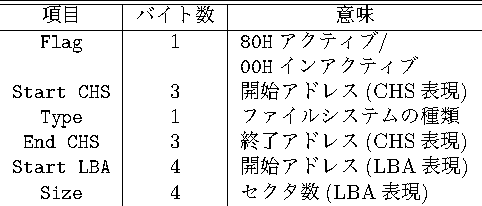
\includegraphics[scale=0.8]
        {../Tbl/partitionTableEntry.pdf}}
    \end{minipage}
    \begin{minipage}{0.34\columnwidth}
      \centerline{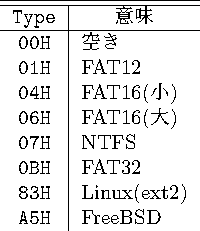
\includegraphics[scale=0.8]
        {../Tbl/partitionTableType.pdf}}
    \end{minipage}
  \end{center}
\end{frame}

%=========================================================================
\begin{frame}
  \frametitle{ブートストラップ(1)}
  \emph{PCの場合を例にブートストラップを説明する.}
  \begin{itemize}
  \item ハードディスクからOSを起動する作業のこと.
  \item OSのカーネルを格納したファイルを見つけてロード・実行する.
  \item PCの製造時にはどんなOSがインストールされるか分からない. \\
    => ブートストラップは後で変更できる必要がある.
  \item 以下に説明する段階を経てOSをブートする.
  \item 以下の方法がPCでは標準的であるが様々な変種がある.\\
    (段階が多い場合,強力なブートマネージャを備えている場合)
  \end{itemize}
\end{frame}

%=========================================================================
\begin{frame}
  \frametitle{ブートストラップ(2)}
  \emph{ハードディスク = ボリュームの場合}
  \fig{scale=0.55}{bootstrapSequence-crop.pdf}
  \begin{itemize}
  \item \emph{IPL(Initial Program Loader)} \\
    \small{PCのROMに格納されており電源ONと同時に動作開始}
  \item ブートローダ(第1段階:Loader1)\emph{512バイト以内} \\
    \small{LBA0に格納されIPLによってロード・実行される.}
  \item ブートローダ(第2段階:Loader2) \\
    \small{ディスク上のどこか連続セクタに格納されLoader1がロード・実行.\\
      サイズに制限がない => 高機能にできる.}
  \item OSのカーネル \\
    \small{ファイルシステムにファイルとして格納されLoader2がロード・実行.}
  \end{itemize}
\end{frame}

%=========================================================================
\begin{frame}
  \frametitle{ブートストラップ(3)}
  \emph{パーティション = ボリュームの場合}
  \fig{scale=0.55}{bootstrapSequenceMulti-crop.pdf}
  \begin{itemize}
  \item \emph{IPL(Initial Program Loader)}
  \item ブートセレクタ・ブートマネージャ(Boot)\emph{446バイト以内} \\
    \small{LBA0(MBR)に格納されIPLによってロード・実行される.\\
    メニューを表示してユーザにOSのパーティションを選択させる.\\
    (勝手に次に進むものもある.)}
  \item ブートローダ(第1段階:Loader1)\emph{512バイト以内} 
  \item ブートローダ(第2段階:Loader2)
  \item OSのカーネル
  \end{itemize}
\end{frame}

%=========================================================================
\begin{frame}
  \frametitle{練習問題(1)}
  \begin{enumerate}
  \item[1.] 次の言葉の意味を説明しなさい.
    \begin{itemize}
    \item 二次記憶装置
    \item 揮発性・不揮発性
    \item 記憶の階層
    \item テープ型装置・ディスク型装置
    \item シーケンシャルアクセス・ランダムアクセス
    \item セクタ・トラック・シリンダ
    \item CHS・LBA
    \item ボリューム
    \item パーティション
    \item MBR
    \item IPL
    \item ブートストラップ
    \end{itemize}
  \end{enumerate}
\end{frame}

%=========================================================================
\begin{frame}
  \frametitle{練習問題(2)}
  \begin{enumerate}
  \item[2.] 次のディスクに付いて答えなさい.
    \begin{quote}
      \begin{tabular}{l l}
        1台全体   & 1,024シリンダ  \\
        1シリンダ & 8トラック      \\
        1トラック & 128セクタ      \\
        1セクタ   & 512バイト
      \end{tabular}
    \end{quote}
    \begin{itemize}
    \item ディスクの容量をセクタ単位で答えなさい.
    \item ディスクの容量をバイト単位で答えなさい.
    \item 最後のセクタのアドレスをLBAで答えなさい.
    \item 最後のセクタのアドレスをCHSで答えなさい.\\
      (但し,C:0以上,H:0以上,S:1以上である.)
    \end{itemize}
  \end{enumerate}
\end{frame}

%=========================================================================
\begin{frame}
  \frametitle{練習問題(3)}
  \begin{enumerate}
  \item[3.] 例示したパーティションテーブルに付いて答えなさい.
    \begin{itemize}
    \item 第1パーティションの位置をLBAで答えなさい.
    \item 第1パーティションのサイズをセクタ数で答えなさい.
    \item 第1パーティションの種類を答えなさい.
    \item 第2パーティションの位置をLBAで答えなさい.
    \item 第2パーティションのサイズをセクタ数で答えなさい.
    \item 第2パーティションの種類を答えなさい.
    \end{itemize}
    \vfill
  \item[4.] PC用の高機能なブートローダGRUBについて調査しなさい.
    \vfill
  \end{enumerate}
\end{frame}

%=========================================================================
%\begin{frame}
%  \frametitle{}
%\end{frame}

\end{document}
